\documentclass[11pt]{article}
\usepackage[margin=1in]{geometry}
\usepackage{booktabs}
\usepackage{graphicx}
\usepackage{float}
\usepackage{longtable}
\usepackage{hyperref}
\title{Ramen TTA -- Experiment Report}
\author{Auto-generated by experiments.py}
\date{2026-08-31 16:58:49}
\begin{document}
\maketitle

\section{Run configuration}
\begin{itemize}

  \item \textbf{date}: 2026-08-31 16:58:49

  \item \textbf{sweep\_run}: False

  \item \textbf{diagnostics\_run}: False

  \item \textbf{tsne\_run}: False

  \item \textbf{device}: cuda

  \item \textbf{num\_result\_rows}: 285

  \item \textbf{datasets}: CIFAR100C, CIFAR10C

\end{itemize}

\section{Average accuracy per algorithm / flag}

Each cell is the mean over all corruption domains of that run's per-domain accuracy (\%). Compare adaptation on/off (NoAdapt vs Tent vs Ramen) and the \texttt{use\_tbn} toggle.


\begin{table}[H]
\centering
\small
\begin{tabular}{llrr}
\toprule
dataset & tta\_algo & off & on \\
\midrule
CIFAR100C & NoAdapt & 37.10 & -- \\
CIFAR100C & Ramen & 46.12 & 46.12 \\
CIFAR100C & Tent & 41.14 & 41.14 \\
CIFAR10C & NoAdapt & 61.36 & -- \\
CIFAR10C & Ramen & 72.63 & 72.63 \\
CIFAR10C & Tent & 66.71 & 66.71 \\
\bottomrule
\end{tabular}

\caption{Mean per-domain accuracy (\%) by dataset, algorithm and use\_tbn.}
\end{table}

\begin{table}[H]
\centering
\small
\begin{tabular}{llrr}
\toprule
dataset & tta\_algo & use\_tbn & avg\_acc \\
\midrule
CIFAR100C & Ramen & False & 46.12 \\
CIFAR100C & Ramen & True & 46.12 \\
CIFAR100C & Tent & False & 41.14 \\
CIFAR100C & Tent & True & 41.14 \\
CIFAR100C & NoAdapt & False & 37.10 \\
CIFAR10C & Ramen & False & 72.63 \\
CIFAR10C & Ramen & True & 72.63 \\
CIFAR10C & Tent & False & 66.71 \\
CIFAR10C & Tent & True & 66.71 \\
CIFAR10C & NoAdapt & False & 61.36 \\
\bottomrule
\end{tabular}

\caption{All runs ranked by average accuracy within each dataset.}
\end{table}

\section{Per-domain accuracy}

\subsection*{CIFAR100C}

\begin{table}[H]
\centering
\small
\begin{tabular}{lrrr}
\toprule
domain & NoAdapt & Ramen & Tent \\
\midrule
glass\_blur & 20.16 & 29.34 & 23.67 \\
gaussian\_noise & 22.83 & 30.50 & 24.87 \\
shot\_noise & 24.42 & 32.77 & 27.03 \\
pixelate & 26.29 & 40.42 & 31.53 \\
elastic\_transform & 29.21 & 36.83 & 31.81 \\
impulse\_noise & 29.58 & 42.80 & 34.49 \\
jpeg\_compression & 33.57 & 39.15 & 37.24 \\
contrast & 35.27 & 51.18 & 43.93 \\
fog & 41.77 & 52.65 & 45.27 \\
motion\_blur & 43.60 & 52.20 & 46.98 \\
defocus\_blur & 43.56 & 52.46 & 49.52 \\
frost & 50.48 & 54.72 & 50.98 \\
snow & 48.91 & 55.23 & 52.63 \\
zoom\_blur & 48.64 & 55.65 & 53.95 \\
brightness & 58.15 & 65.96 & 63.24 \\
\bottomrule
\end{tabular}

\caption{CIFAR100C: per-domain accuracy (\%) by algorithm (use\_tbn=off), sorted ascending.}
\end{table}

\begin{table}[H]
\centering
\small
\begin{tabular}{lrrr}
\toprule
domain & NoAdapt & Ramen & Tent \\
\midrule
glass\_blur & 20.16 & 29.34 & 23.67 \\
gaussian\_noise & 22.83 & 30.50 & 24.87 \\
shot\_noise & 24.42 & 32.77 & 27.03 \\
pixelate & 26.29 & 40.42 & 31.53 \\
elastic\_transform & 29.21 & 36.83 & 31.81 \\
\bottomrule
\end{tabular}

\caption{CIFAR100C: 5 weakest corruption domains (by Tent).}
\end{table}

\subsection*{CIFAR10C}

\begin{table}[H]
\centering
\small
\begin{tabular}{lrrr}
\toprule
domain & NoAdapt & Ramen & Tent \\
\midrule
gaussian\_noise & 38.66 & 60.84 & 38.60 \\
shot\_noise & 42.59 & 63.35 & 41.56 \\
impulse\_noise & 42.75 & 56.13 & 45.53 \\
glass\_blur & 43.91 & 64.11 & 56.22 \\
pixelate & 51.88 & 65.18 & 60.55 \\
jpeg\_compression & 58.58 & 67.32 & 63.86 \\
elastic\_transform & 61.97 & 71.95 & 69.57 \\
motion\_blur & 66.68 & 77.26 & 72.63 \\
fog & 68.85 & 78.38 & 73.94 \\
contrast & 67.07 & 79.68 & 75.54 \\
defocus\_blur & 72.61 & 77.07 & 78.05 \\
zoom\_blur & 71.69 & 78.84 & 78.18 \\
snow & 73.78 & 80.79 & 79.68 \\
frost & 75.69 & 80.42 & 79.85 \\
brightness & 83.62 & 88.14 & 86.84 \\
\bottomrule
\end{tabular}

\caption{CIFAR10C: per-domain accuracy (\%) by algorithm (use\_tbn=off), sorted ascending.}
\end{table}

\begin{table}[H]
\centering
\small
\begin{tabular}{lrrr}
\toprule
domain & NoAdapt & Ramen & Tent \\
\midrule
gaussian\_noise & 38.66 & 60.84 & 38.60 \\
shot\_noise & 42.59 & 63.35 & 41.56 \\
impulse\_noise & 42.75 & 56.13 & 45.53 \\
glass\_blur & 43.91 & 64.11 & 56.22 \\
pixelate & 51.88 & 65.18 & 60.55 \\
\bottomrule
\end{tabular}

\caption{CIFAR10C: 5 weakest corruption domains (by Tent).}
\end{table}

\section{Per-domain accuracy (figure)}

Bars sorted ascending; dashed line = that run's own average; red bars are domains below the average (dragging the total down).


\begin{figure}[H]\centering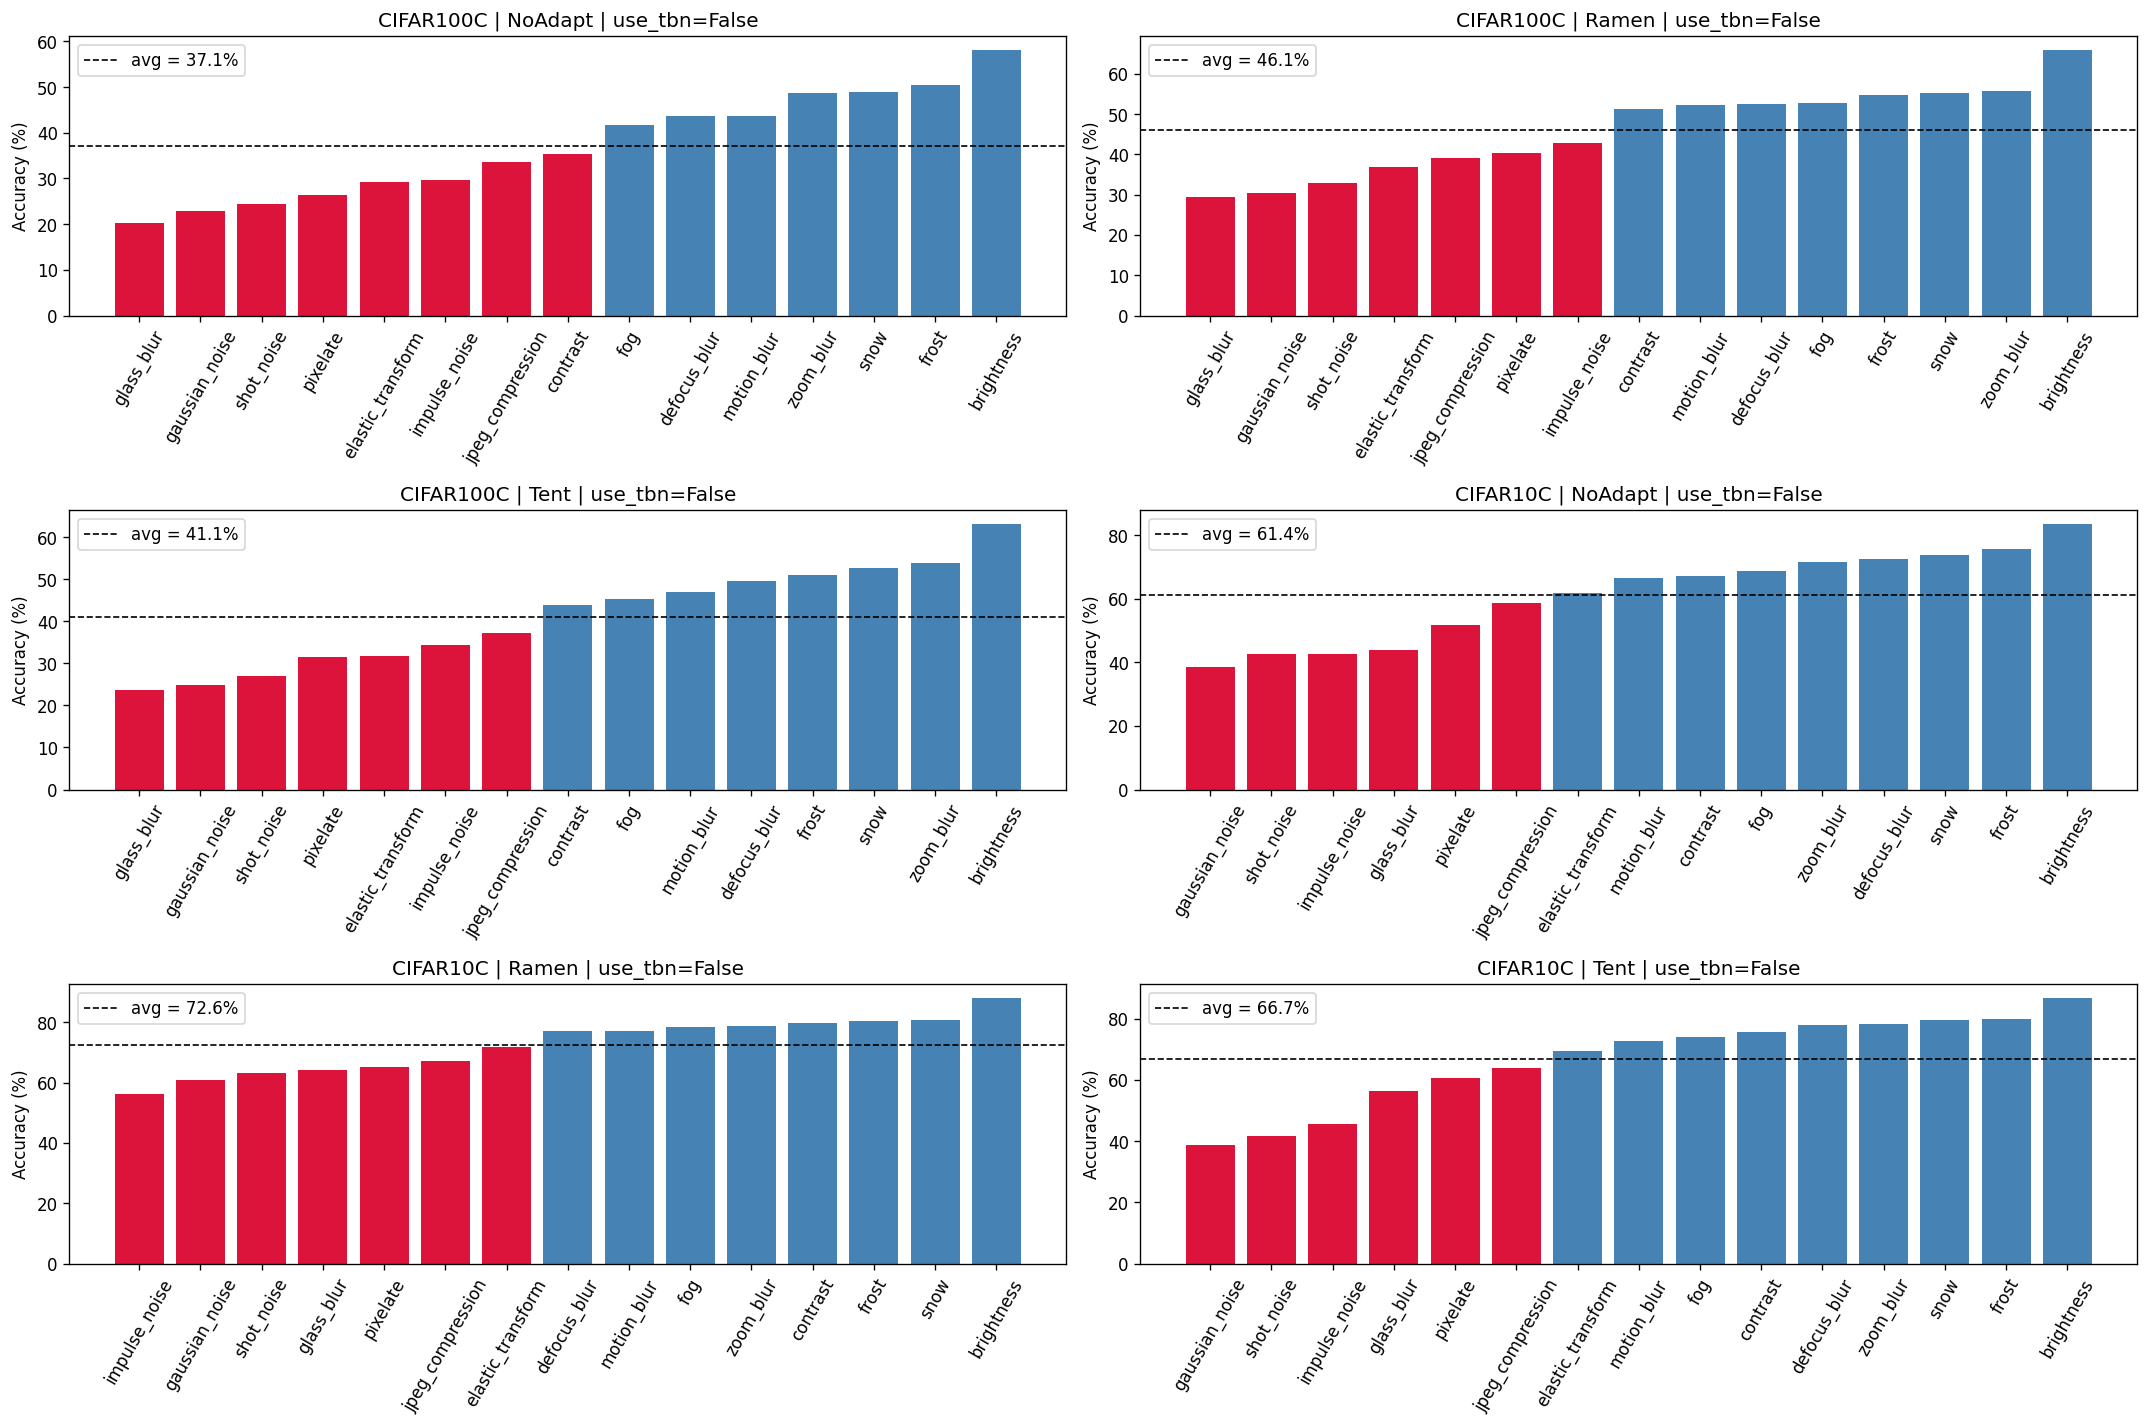
\includegraphics[width=\textwidth]{figures/domain_accuracy.png}\caption{Per-domain accuracy, per (dataset, algorithm).}\end{figure}

\end{document}
